% generated by src/r2/paper_assets (make_paper_assets.py figures); do not edit by hand
% provenance: fig2_model generated by src/r2/paper_assets on 2026-10-15 04:07 from data/r2/tables/
%   fit_source_parameters.csv (modified 2026-10-14 19:28): universe = global, fit_id = family_hb_nuts, parameter in {alpha, beta}
%   modes_bridge.csv (modified 2026-10-14 20:11): role = primary_estimate, mode = 1 (second mode); coords = centred, proposal = mvn
%   modes_simulation_replicates.csv (modified 2026-10-14 20:12): simulator = faithful_cc (design-faithful); dominant_is_truth, dominant_strong_realised_fdr
%   modes_simulation.csv (modified 2026-10-14 20:12): stratum in {dominant_is_truth, dominant_not_truth, all}; quantity in {dominant_strong_realised_fdr_mean, dominant_strong_claimed_bfdr_mean, p_dominant_is_truth}; simulator = faithful_cc (primary); faithful_cc_strat and fixed_masks (sensitivity, caption only)
%   modes_faithful_design.csv (modified 2026-10-14 20:12): quantity = n_edges_cc_observed, sim_label in {immune_cc, global_cc}: ratio_sim_mean_to_real (share of the real motif/coexpression-observed edges)
%   fit_modes.csv (modified 2026-10-14 19:29): w_T and w_2 (= class B_LIT; class order T, N, B_LIT, B_MOTIF as in fit_class_weights) of optimum 0 and 1
\begin{figure}[tbp]
  \centering
  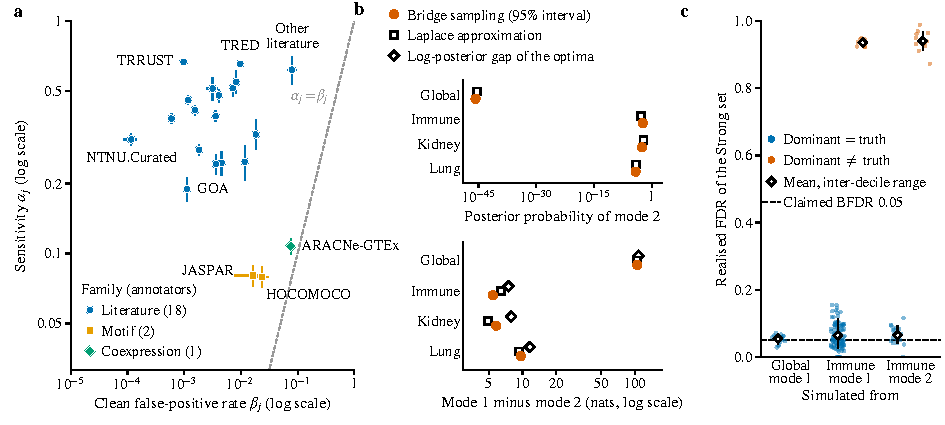
\includegraphics[width=\textwidth]{fig2_model.pdf}
  \caption{\textbf{Family-HB parameters and posterior modes.} (a) Annotator sensitivity $\alpha_j$ against clean false-positive rate $\beta_j$ (posterior means with 95\% credible intervals, global universe, NUTS) for the 21 held-in annotators (18 literature); the dashed diagonal is $\alpha_j=\beta_j$, which the parametrisation excludes. Sensitivities range from 0.08 to 0.67 and false-positive rates from 0.00012 to 0.079. (b) Mode 1 is the dominant posterior mode of each universe fit and mode 2 the second (in the global and immune fits, whose class weights are stored for both modes, mode 2 approximately exchanges the weights of the true class and the literature-burst class). Top: posterior probability of mode 2 by bridge sampling (filled; Monte Carlo 95\% interval) and by Laplace's method (open squares). Bottom: mode 1 minus mode 2 in log posterior mass (bridge sampling, filled; Laplace's method, open squares) and the log-posterior gap of the two optima (diamonds). Values and ranges in Table~\ref{tab:fit}. (c) Mode-selection simulation from the fitted model with the design-faithful simulator (data simulated at the parameters of the indicated mode with the real literature observation masks and the motif/coexpression masks rebuilt from the simulated literature reports, as in the evidence builder; the simulated data contain 59\% (immune) and 62\% (global) of the real number of motif- or coexpression-observed edges; refitted by multi-start MAP): realised false discovery rate of the Strong set for replicates whose dominant mode is or is not the truth mode (points: replicates; diamonds: mean with inter-decile range over replicates; dashed line: claimed BFDR 0.05); global universe, truth = mode 1: dominant mode is the truth mode in all 20 replicates, mean realised FDR 0.05; immune universe, truth = mode 1: dominant mode is the truth mode in 93 of 100 replicates, mean realised FDR 0.06 when it is and 0.94 when it is not; immune universe, truth = mode 2: dominant mode is the truth mode in 18 of 30 replicates, mean realised FDR 0.06 when it is and 0.94 when it is not. Sensitivity, probability that the dominant mode is the truth mode with every observation mask fixed at the real one: global universe 0.70, immune universe 0.68, immune universe (truth = mode 2) 0.77; with class weights that depend on the literature-mask stratum: global universe 1.00, immune universe 1.00, immune universe (truth = mode 2) 0.97 (Supplementary Table~\ref{tab:S-modes-sim}). The bridge-sampling estimates in (b) and panel (c) are post hoc (defined after the held-out data had been examined; no held-out data are used).}
  \label{fig:model}
\end{figure}
